\documentclass[11pt]{article}

\usepackage[margin=1in]{geometry}
\usepackage{fancyhdr}
\pagestyle{fancy}
\usepackage{amsmath}
\usepackage{amssymb}
\usepackage{fancyhdr}
\pagestyle{fancy}
\usepackage{amsmath}
\usepackage{amssymb}
\usepackage{multirow}
\usepackage{array}
\usepackage{tikz}
\usetikzlibrary{calc,trees,positioning,arrows,fit,shapes,calc}

\lhead{Propositional Logic}
\chead{Asli Akalin | Note 1}
\rhead{Summer 2018}


\begin{document}
\section*{Terms and Notation}
\begin{enumerate}

\item
Definifitons
\begin{enumerate}
\item 
Axiom: known to be true statements, asserted as True, aren't proven.
\item 
Proposition: statements that have a truth value of either true or false, should be proven. We use axioms to determine truth values of propositions.
\item 
Propositional form: can create larger statements by putting propositions together using logical symbols, (i.e  $\neg (({P_1} \vee {P_2}) \wedge ({P_3} \vee {P_4}))$
\item
Tautology: statements that are always true, regardless of its variables' truth values. For example, $(P \vee {\neg P})$ is always true whether P is True or False.
\item
Contradiction: statements that are always false, regardless of its variables' truth values. For example, $(P \wedge {\neg P})$ is always false whether P is True or False.
\item
Logical Equivalence: $A \equiv \neg (({P_1} \vee {P_2}) \wedge ({P_3} \vee {P_4}))$ shows that A and the given complex proposition represent the same statement and their truth values are the same. Like an equal sign in logic notation (i.e can write $2 + 6 + 8 = 8 + 8 = 16$). Since we don't know the value of the proposition during the proof, we can't use the equal sign but we can step by step simplify the original statement by finding its logical equivalent at each step.
\end{enumerate}

\item
Logical Symbols
\begin{enumerate}
\item not: $\neg P$, unary operation
\item and: $P \wedge Q$, binary operation
\item or: $P \vee Q$, binary operation
\item implies: $P \Rightarrow Q$, binary operation, $(P \Rightarrow Q) \equiv {\neg P} \vee Q$
\item logical equivalence: $A \equiv B$ or $(A \Rightarrow B) \wedge (B \Rightarrow A)$ or $(A \Leftrightarrow B) $ can all be used to show logical equivalence of A and B
\end{enumerate}
\end{enumerate}

\section*{Distributive Laws and Inference}
\begin{enumerate}
\item Distributing Negation: De Morgan's Laws
\begin{enumerate}
\item $\neg {\neg P} \equiv P$
\item $\neg (P \wedge Q) \equiv ({\neg P} \vee {\neg Q})$
\item $\neg (P \vee Q) \equiv ({\neg P} \wedge {\neg Q})$
\item $ \neg (\forall x$ $P(x)) \equiv \exists x$ ${\neg P(x)}$
\item $ \neg (\exists x$ $P(x) \equiv \forall x$ ${\neg x P(x)}$
\end{enumerate}

\item Distributing Conjunctive and Disjunctive Forms
\begin{enumerate}
\item $P \wedge (Q \vee R) \equiv (P \wedge Q) \vee (P \wedge R)$, similarly $P \wedge (Q \wedge R) \equiv (P \wedge Q) \wedge (P \wedge R) \equiv P \wedge Q \wedge R$
\item $P \vee (Q \wedge R) \equiv (P \vee Q) \wedge (P \vee R)$, similarly $P \vee (Q \vee R) \equiv (P \vee Q) \vee (P \vee R) \equiv P \vee Q \vee R$
\end{enumerate}

\newpage
\item Distributing Quantifiers:\\
Remember the quantifier definitions:\\
$\forall x, P(x) \equiv P({x_1}) \bigwedge P({x_2}) \bigwedge P({x_3}) \bigwedge $ ... for all ${x_i}$ values \\
$\exists x, P(x) \equiv P({x_1}) \bigvee P({x_2}) \bigvee P({x_3}) \bigvee $ ... for all ${x_i}$ values
\begin{enumerate}
\item $\forall x, (P(x) \wedge Q(x)) \equiv (\forall x$ $P(x)) \wedge (\forall x$ $Q(x))$
\item $\exists x, (P(x) \vee Q(x)) \equiv (\exists x$ $P(x)) \vee (\exists x$ $Q(x))$
\end{enumerate}
(Exercise: show using the quantifier definitions why is this so. Reference: Discussion 1b, Q1)

\item Inference: we can simplify statements using known truth values:
\begin{enumerate}
\item $T \wedge P \equiv P$
\item $F \wedge P \equiv F$
\item $T\vee P \equiv T$
\item $F \vee P \equiv P$
\item $F \Rightarrow P \equiv T$
\item $T \Rightarrow P \equiv P$
\end{enumerate}

\item Contrapositive and Converse of $P \Rightarrow Q$
\begin{enumerate}
\item Contrapositive: ${\neg Q} \Rightarrow {\neg P}$. Logical equivalent of $P \Rightarrow Q$\\
(Proof: $P \Rightarrow Q \equiv \neg P \vee Q$  and $(\neg Q \Rightarrow \neg P) \equiv Q \vee \neg P$ thus $\neg P \vee Q \equiv Q \vee \neg P$)
\item Converse: $Q \Rightarrow P$
\end{enumerate}
\end{enumerate}

\section*{Understanding Implication}
\begin{enumerate}
\item $P \Rightarrow Q$: If P, then Q or P implies Q. Gives a condition/background for Q.
\item 
The following rule is useful to negate complex propositions that include implications. To negate such statements, first get rid of the implication by using $(P \Rightarrow Q) \equiv {\neg P} \vee Q$\\
(Exercise: use a truth table to show these two statements are indeed equivalent)
\item An implication is only false if P is true and Q is false. Follow the next example to understand why is this so.
\item Class example: P(x): student x is in cs70 discussion, Q(x): "student x is taking cs70." \\ Consider then "if P, then Q" true (i.e it would make intuitive sense in this example)?
\begin{enumerate}
\item if student is in class, and she is taking cs70: $T \Rightarrow T
 \equiv T$  \\(makes sense since she showed up for the discussion section for her class)
 \item if student is not in class, and she is taking cs70: $F \Rightarrow T  \equiv T$ \\ (makes sense since she might be in a different discussion section for the class)
 \item if student is not in class, and she is not taking cs70: $F \Rightarrow F
 \equiv T$ \\ (makes sense since if she is not taking the class, there is no reason for her to be in discussion)
 \item it would only not make sense if the student was in class but she is not enrolled in cs70: $T \Rightarrow F \equiv F$ (why would she come to discussion for a class she is not enrolled in? Her presence in the class cannot imply that she is not taking this class)
\end{enumerate}
\item Approach the LHS of implication as "background" or "hypothesis" the statement is going to be built on, RHS of implication as the "result" or "conclusion" based on the background set by the LHS. If the hypothesis is wrong to begin with (i.e if our background information is not accurate) we can't conclude any information about the given result, it can be true or false. We can conclude info about RHS if LHS is True, which means once LHS is True, the truth value of the implication depends entirely on RHS. (look at "Distributive Laws and Inference" Part 3, e and f for the formal statements.)
\item The main idea is to evaluate Q on the basis of whether P holds or not.

\end{enumerate}


\section*{Truth Tables}
\begin{displaymath}
\begin{array}{|ccc|c|c|}
\hline
P & Q & R & P \wedge (Q \vee R) & (P \wedge Q) \vee (P \wedge R)\\ % Use & to separate the columns
\hline % Put a horizontal line between the table header and the rest.
T & T & T & T & T\\
T & T & F & T & T\\
T & F & T & T & T\\
T & F & F & F & F \\
F & T & T & F & F \\
F & T & F & F  & F\\
F & F & T & F &  F\\
F & F & F & F & F\\
\hline
\end{array}
\end{displaymath}
\begin{enumerate}
\item Use truth tables to get truth values of complex propositions by listing all possible input values of their variables.
\item We specify functions by specifying their outputs for each possible input.
\item If final columns of two truth tables are the same, then two statements are logical equivalent of each other.
\item Tautologies have a last column of all True values, they are true for all possible assignments of variables.
\item  Contradictions have a last column of all False values, they are false for all possible assignments of variables.
\end{enumerate}


\section*{Quantifiers}
\begin{enumerate}
\item 
$\forall x$: universal quantifier, "for all x" \\
$\forall x, P(x) \equiv P({x_1}) \bigwedge P({x_2}) \bigwedge P({x_3}) \bigwedge $ ... for all ${x_i}$ values
\item
$\exists x$: existential quantifier, "there exists x", can refer to one or more x (at least one)\\
$\exists x, P(x) \equiv P({x_1}) \bigvee P({x_2}) \bigvee P({x_3}) \bigvee $ ... for all ${x_i}$ values
\end{enumerate}

\newpage
\section*{Graphing Technique for Evaluating Quantifiers}
\begin{enumerate}
\item
\begin{figure}[ht]
\centering
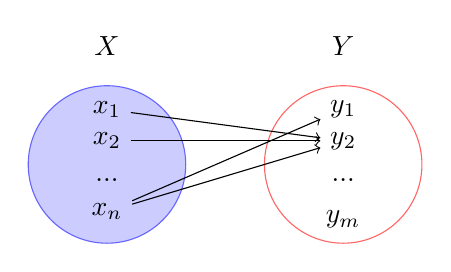
\begin{tikzpicture}
    % draw the sets
    \filldraw[fill=blue!20, draw=blue!60] (-1.5,0) circle (1cm);
    \filldraw[fill=red!0, draw=red!60] (1.5,0) circle (1cm);

    % the texts
    \node at (-1.5,1.5) {$X$};
    \node at (1.5,1.5) {$Y$};

    % the points in the sets (here I just create nodes to use them later on to position
    % the circles and the arrows
    \node (x1) at (-1.5,0.7) {$x_1$};
    \node (x2) at (-1.5,0.3) {$x_2$};
     \node (x3) at (-1.5,-0.2) {$...$};
    \node (x4) at (-1.5, -0.6) {$x_n$};
    \node (y1) at (1.5,0.7) {$y_1$};
    \node (y2) at (1.5,0.3) {$y_2$};
    \node (y3) at (1.5,-0.2) {$...$};
    \node (y4) at (1.5,-0.7) {$y_m$};

    % draw the arrows
    \draw[->] (x1) -- (y2);
    \draw[->] (x2) -- (y2);
    \draw[->] (x4) -- (y2);
    \draw[->] (x4) -- (y1);

\end{tikzpicture}
\caption{Mapping diagram of ($\forall x$, $\exists y$) for some statement P(x,y)}
\end{figure}
\begin{enumerate}
\item $\forall x$ makes sure all x are selected in set of x, for each $x_i$ there will be (at least one) arrow going out, this set of X is all selected. Therefore we can say for all x, there at least some y (one or more) that makes P(x,y) True.
\item $\forall x$, $\exists y$ does not guarantee that all y values in set Y will have a corresponding x value to make statement P(x,y) true, for example in this example $y_m$ doesn't have a x pair. \newline$\forall x$, $\exists y$ means all $x_i$ can point at the same y value, or different y values.
\item Only thing known for certain here is that you can pick any x value, and you can find a specific y' value for that x make $P(x, y')$ correct, $y'$ can be the same for all x or each x might use different y values.
\end{enumerate}



\begin{figure}[ht]
\centering
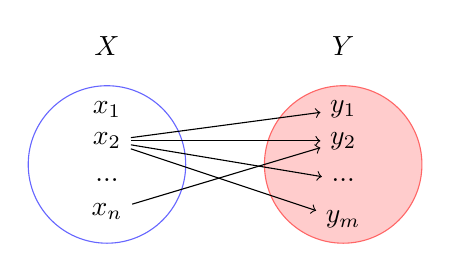
\begin{tikzpicture}
    % draw the sets
    \filldraw[fill=blue!0, draw=blue!60] (-1.5,0) circle (1cm);
    \filldraw[fill=red!20, draw=red!60] (1.5,0) circle (1cm);


    % the texts
    \node at (-1.5,1.5) {$X$};
    \node at (1.5,1.5) {$Y$};

    % the points in the sets (here I just create nodes to use them later on to position
    % the circles and the arrows
    \node (x1) at (-1.5,0.7) {$x_1$};
    \node (x2) at (-1.5,0.3) {$x_2$};
     \node (x4) at (-1.5,-0.2) {$...$};
    \node (x5) at (-1.5, -0.6) {$x_n$};
    \node (y1) at (1.5,0.7) {$y_1$};
    \node (y2) at (1.5,0.3) {$y_2$};
    \node (y3) at (1.5,-0.2) {$...$};
    \node (y4) at (1.5,-0.7) {$y_m$};

    % draw the arrows
    \draw[->] (x2) -- (y1);
    \draw[->] (x2) -- (y2);
    \draw[->] (x2) -- (y3);
    \draw[->] (x2) -- (y4);
    \draw[->] (x5) -- (y2);

\end{tikzpicture}
\caption{Mapping diagram of ($\exists x$, $\forall y$) for some statement P(x,y)}
\end{figure}
\item 
\begin{enumerate}
\item $\exists x$ makes sure that there is (at least) one x, x' such that it can be paired with every single y value to make the statement P(x,y) correct. In this case the guarantee is that the set Y is covered.
\item $\exists x$, $\forall y$ doesn't mean there is only one x that can make P(x,y) correct. For example in this example $y_2$ can be paired with $x_2$ or $x_n$. 
\item However $\exists x$, $\forall y$ does enforce that if we took let's say $y_11$, $y_167$ and $y_4$, we would be able to find at least one specific x that can be paired with all those values to make P(x,y) correct.
\end{enumerate}
\item Be careful with what the order of quantifiers guarantee and what they might satisfy in certain cases!! For example $\exists x$, $\forall y$ might mean that there are two x values $x_i$ and $x_j$ such that all y values can be paired with either to make P(x,y) but it does not guarantee that some x, $x_k$ will have a corresponding y value to make P(x,y) correct. 

\end{enumerate}
\newpage
\section*{Useful Notes}
\begin{enumerate}
\item 
While converting an English sentence to propositional form, use quantifiers to define the set that the sentence applies to; use implications LHS to define the conditions or background info outlined in the sentence for statement to hold.
\begin{enumerate}
\item "every integer," "real numbers x, y" can be converted $\forall x \in Z$ and 
${x,y}\in R$
\item "positive integer x, ..." can be converted as $\forall x \in Z, x>0 \Rightarrow$ ... It might be easier to interpret these phases as "for all integers x, if x is positive, then ..."
\end{enumerate}
Key Point: If you are not sure when to use quantifiers and when to use implications, look for a way to rephrase the sentence using "if ..., then ..." to see if you can use implications. "if x is positive, then..." or "if x and y are distinct, then ..."
\item To show something does not exist you can use two main structures:
\begin{enumerate}
\item "for all possible things, it cannot happen" : using $\forall$ and $\neq$
\item NOT "there exits a case that it can happen": using $\neg $ ($\exists$ and =)
\end{enumerate}
Key Point: these two structures are essentially the same if you distribute the negation of the second structure. Don't forget that "NOT" should cover the entire statement saying there is a case that it is possible. We are trying to say that there cannot even be a single case that it can happen.

\item To show that there is only one of something, we argue that if there were multiple things that could fix the given statement's specifications, they would have to be the same. In simple terms, to show there is only one integer that is equal to 3, we can say: \\ $\exists x \in Z, ((x = 3) \wedge (\forall y \in Z = 3)) \Rightarrow (x = y) $ which says if there's an x that equals to 3, all other possible y values that equal 3 has to be equal to x.

\item  "can find" means "there exists"
\item  "a between x and y" can be shown as $ (x < a <y) \vee (y<  a <x)$
\item "distinct x and y" means $x \neq y$
\end{enumerate}
\newpage
\section*{Review Questions}
\begin{enumerate}
\item If chemical plant pollutes river, fish die. If fish die, did the chemical plant pollute water?
\item Are these statements logically equivalent? a) If plant pollutes, fish die. b) if fish die, plant pollutes.
\item $(\forall x \in Z) (\exists y \in Z) (y > x)$? $(\exists y \in Z) (\forall x \in Z)  (y > x)$?
\end{enumerate}

\section*{Answers}
\begin{enumerate}
\item First, define P(x) as "chemical plant pollutes water" and Q(x) as "fish die." We have "if chemical plant pollutes river, fish die" known to be True: $P(x) \Rightarrow Q(x) \equiv T$. The question asks if fish die, $Q(x) \equiv T$, did the chemical plant pollute the water, $P(x) \equiv T$? Using the implication definition, we know that $P(x) \Rightarrow Q(x)$ and $Q(x)$ True can mean $P(x)$ is either True or False, since $T \Rightarrow T$ and $F \Rightarrow T$ both evaluate to T. So, by knowing fish died and knowing one of the reasons fish dies is chemical plant pollution, we cannot conclude that chemical plant polluted the water. Intuitively, we can see that fish might have died from a different reason. So, the fact that fish died does not necessarily mean chemical plant pollutes water. 
Key Point: P is sufficient for Q (proving P allows you to conclude Q is true, since if $P \rightarrow Q$ is true and P is true, Q has to be true) but Q is necessary for P (for P to be true Q is required to be true, because if $P \rightarrow Q$ is true and Q is false, P has to be false to make the implication still be true).
\item They are not logically equivalent. They are the converse of each other. If plant pollutes, fish will die for sure, so if fish are alive it is safe to say plant is not polluting. But fish can die for many reasons, so just because fish die we can't be certain that plant is polluting. (Exercise inception: prove these explanatory sentences using logic language.)
\item Frist statement says for each integer x, we can find at least one integer y that is bigger than x. True since there is always a bigger integer. Second statement says that there is one integer, call it y, such that it is bigger than all integers. False since there is no "biggest integer"
\end{enumerate}

\end{document}